\documentclass[]{article}
\usepackage{graphicx}
\usepackage{color}

\newcommand{\answer}[1]{\textcolor{red}{\bf #1}}

\begin{document}

%%%%%%%%%
\section*{Population Genetics}

\begin{enumerate}
\item What’s the highest possible frequency of heterozygotes at a single biallelic locus at HWE?

\answer{0.5}
\item The frequency of A1 in a population is 0.7.  A troll eats half the homozygous A1A1 individuals, then leaves.  After one generation of completely random mating, is the population at HWE?

\answer{yes}
\item  In a population at Hardy-Weinberg Equilibrium (HWE) at the A locus, there are six times as many heterozygous A1A2 individuals as homozygous A2A2 genotypes.  What is the frequency of A1?

\answer{0.75}
\item The frequency of the R allele (at a locus with alleles R and r) in a population at HWE is 0.4.  If you sample 500 individuals from this population, what is the frequency of the rr genotype? 

\answer{0.36}
\item  In an infinite size diploid neutral population mating randomly with frequency of the MM genotype of 4\%, what is the frequency of the m allele (the locus is biallelic)?


\answer{0.8}
\item  Can genetic drift lead to evolution?  Why or why not?

\answer{yes, changes allele freqs.}

\item Farmer Jones is trying to eliminate a recessive dwarf allele at the dwarfus locus from his pea crop. In 2010, his fields yielded 9\% dwarf plants. You may assume that his population in 2010 is in HWE. When planting his 2011 crop, the farmer used only the seeds from the tall plants of the previous year. Tall (D) is dominant to dwarf (d). If there is no further selection, what do you predict will be the frequency of dwarf pea plants in the 2011 crop?

\answer{5.3\%. Genotype freqs are 9\%dd 42\%Dd and 49\% DD before selection. Farmer kills all dd. New genotype freqs after selection are 0.42/0.91= 46.15\%Dd 54.85\%DD and 0\%dd. So new allele frequency of d is 0.231 and new frequency of dd in next generation are $0.231^2=5.2\%$}

\end{enumerate}

%%%%%%%%%
\section*{Gene Expression}
\begin{enumerate}
\item  If I told you that a mutant had a fully functional copy of the mutant gene, with no evidence of mutations in the coding sequence or the promoter, but cDNA for the gene was almost never observed, what mechanisms could explain this result?

\answer{possible answers include: mutations in enhancer, RNAi, epigenetic modifications }
\item The transcription of gene TTFN (terrible transcription factor nine) is activated when two other transcription factors (A and B) interact to recruit a co-activator X. A,B, and X combine to create an enhanceosome upstream of TTFN.  Draw a diagram of the interaction between these genes during transcription.   

\answer{AB bound to enhancer, DNA looping over so AB interact with promoter of TTFN and polymerase}
\item You suspect that a gene is downregulated due to epigenetic modification. Explain how you would show this.

\answer{e.g. bisuflite or DNAse sequencing}

\item If I knock-down a gene using RNAi, will I still be able to: b. make cDNA? PCR amplify the gene?
\answer{no cDNA but yes PCR } 

\end{enumerate}

%%%%%%%%%
\section*{Genomics}
\begin{enumerate}
\item  What is the fate of most gene duplicates?

\answer{loss or pseudogenization}

\item Given the tree in figure \ref{fig:TREE} for a gene family in the species chimera, dragon, unicorn, dolphin, and mermaid, answer the following questions:
\begin{enumerate}
%\item If I create a nonsense mutation in dragon1, is it likely to have an effect? Why or why not?
\item Is chimera2 a paralog or ortholog of chimera1?

\answer{paralog}
\item Is chimera2 an ortholog or paralog of dolphin1?

\answer{ortholog}
\item What is a likely explanation for why there is only one copy of the gene in mermaid?

\answer{gene loss}
\item If dragon1 is expressed in the wings and dragon2 is expressed in the tail, but chimera2 is expressed throughout the body, what kind of process explains the extra copies in dragon?

\answer{subfunctionalization}
 \item Explain the C-Value paradox.

\answer{That there is no correlation between the complexity of an organism and its genome size. Currently thought to be due to the expansion of transposable elements and not an increase in the number of genes.}
\item Two genes are found to have the same function but in different tissues. They show extremely similar sequence. What process likely explains this result?

\answer{ Gene duplication and subfunctionalization.}
\end{enumerate}

\begin{figure}[here]
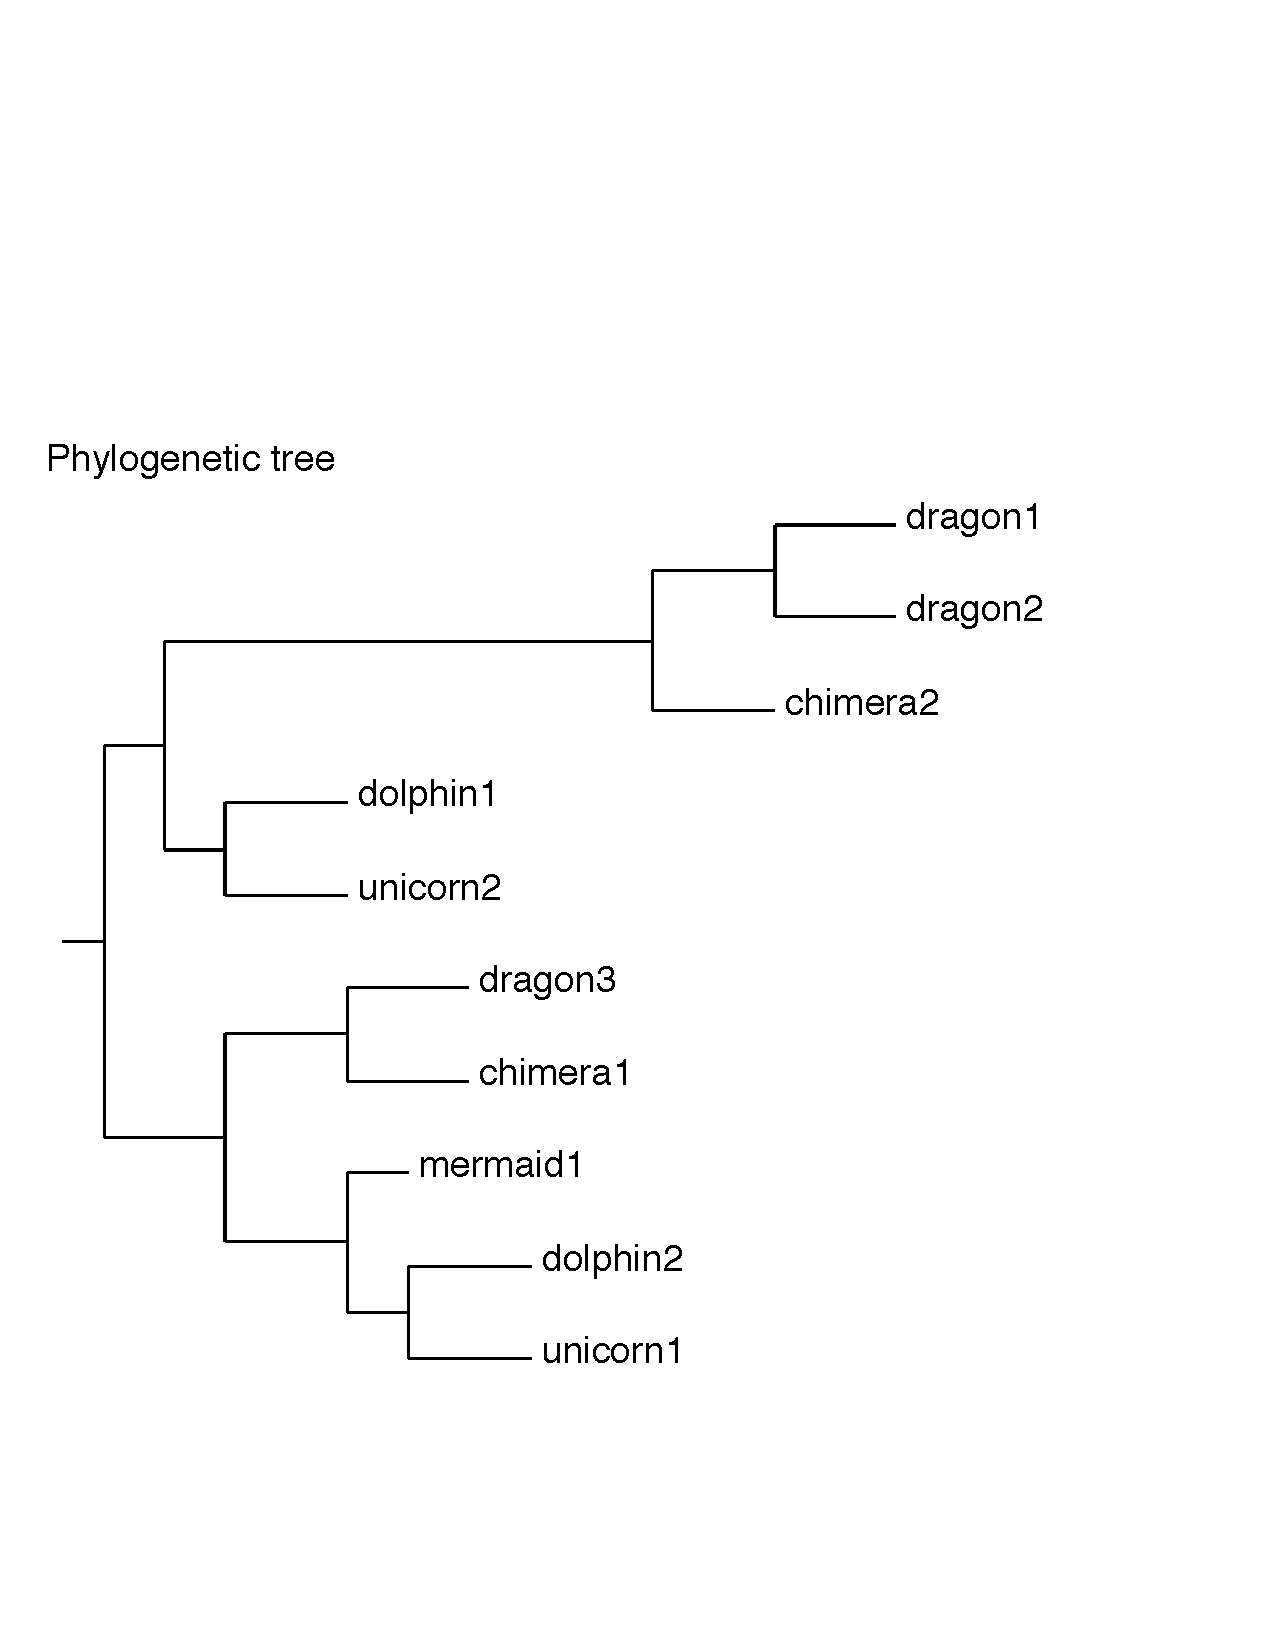
\includegraphics[width=12cm]{faketree.pdf}
\caption{A phylogenetic tree of a fake gene family}
\label{fig:TREE}
\end{figure}
\pagebreak

\item What is synteny and why is it useful?

\answer{similar gene order across species due to ancestry. useful in figuring out function and orthology} 

\item Maize is the second largest plant genome sequenced to date. Given how easy it is to produce sequence data, why haven’t other large genomes been sequenced and assembled?

\answer{repetitive sequence makes assembly difficult and big genomes have lots of repeats}

\item Sorghum chromosome 4 has the gene order  B-C-E-F-G-H-J-K-L.  Maize chromosome 2 has a region with sequence that looks like B2-C2-J2-I2-H2-G2-F2-E2-K2-L2 and maize chromosome 6 has a sequence that looks like R1-S1-F3-F1-T1.  
\begin{enumerate}
\item Which gene in maize would is the likely ortholog of the Sorghum F gene?  Why?

\answer{F2 because of synteny}

\item How many frameshift mutations are required to explain the difference between maize chromosome 2 and Sorghum chromosome 4 ?
\answer{0, it's an inversion} 

\item My PCR In Sorghum uses a forward primer that starts in gene C and ends in Gene E.  Will this PCR work in maize?  Why or why not? 

\answer{Not likely.  If the primer overlaps the breakpoint of the inversion, that sequence will not exist in maize because of the rearrangement.  If the rearrangement breakpoint does not include the primer, it is still likely to fail because of the size of the fragment and the change in sequence orientation.}

\item The Sorghum F gene is an enzyme with an active site coded for by the codons UGC-ACC.  Show a transversion that would generate a nonsense mutation at one of these codons. 
	
\answer{UGC to UGA}

\end{enumerate}
\end{enumerate}

%%%%%%%%%
\section*{Transposable Elements}
\begin{enumerate}
\item Which class of TEs would you expect to make up the largest part of the genome in plants? How about in \emph{Drosophila}? Why?

\answer{ retros in both as they are copy and paste }
\item The maize gene FLX (fluxocapacitor) makes corn kernels sprout puffy white hair (like Christopher Lloyd). Near FLX is a nonautonomous Ds element. If I cross a plant homozygous for functional FLX (FLX+) and presence of the Ds (Ds+) with an inbred plant that has nonfunctioning FLX, no Ds, but an active autonomous Ac element. Draw the phenotype of each parent and the phenotype and genotype of some possible progeny.

\answer{parent 1 smooth kernels, parent 2 kernels with poofy white hair. offspring will likely be puffy white hair with patches of smooth, or smooth with patches of poofy white hair. some may also be all poofy white hair if TE never jumps.}

\end{enumerate}

\section*{Quantitative Genetics}
\begin{enumerate}
\item Yumminess in soybean has a narrow-sense heritability of 0.05\%.  Is it fair to conclude that yumminess has very little genetic basis?  Why or why not? \\
\answer{no. hereitability tells you what \% of variation is due to genes, not whether the trait is genetic}
\end{enumerate}
\end{document}
